% ============================================================
%  CHAPTER 1 — General Context
% ============================================================

% ── Confidentiality warning box ──
\begin{tcolorbox}[
  enhanced, colback=accentgold!8, colframe=accentgold,
  arc=3pt, boxrule=0.8pt, left=10pt, right=10pt, top=8pt, bottom=8pt,
  title={\bfseries\small IMPORTANT CONFIDENTIALITY WARNING},
  fonttitle=\color{chaptercolor},
  before skip=0pt, after skip=20pt
]
\small
This report is an Oracle internal document. It is strictly confidential.
However, Soukaina Bouhsissin and the examiners, as members of the
ENSAM pedagogical team in charge of supervising this project,
are authorized to consult it for the sole purpose of evaluating the author.
Any use outside of this context is prohibited. If you have obtained a copy
of this report without it being explicitly intended for you by the author,
please delete it and report back to the author immediately. In addition,
the examples described in this report are for illustrative purposes only
and do not reflect Oracle's actual business activities.
\end{tcolorbox}

\chapter{General Context}

% ──────────────────────────────────────────
\section{Introduction}
% ──────────────────────────────────────────

In today's world, businesses, technology companies, and the public sector
rely on databases to store their data, while utilizing cloud services to manage
their IT infrastructure and other essential tools such as ERP, CRM, SCM, EPM,
and SPM\@. These technologies have taken a crucial role, making it inconceivable
to function without them.

Oracle, a leading US multinational computer technology corporation, not only
employs these tools in its day-to-day operations but also creates and provides
them to customers. Moreover, the company places a high value on innovation and
ensuring customer satisfaction.

% ──────────────────────────────────────────
\section{Presentation of the Host Organization}
% ──────────────────────────────────────────

  % ── 1.2.1 ──
  \subsection{Oracle Corporation}

  Oracle Corporation is a tech company with headquarters in Austin, Texas.
  In 1977, Larry Ellison, Bob Miner, and Ed Oates founded Oracle Corporation,
  then called Software Development Laboratories (SDL).

  The company first focused on creating Oracle Database, a relational database
  management system (RDBMS), that became its flagship product. Enterprise
  software, cloud computing, hardware systems, and consulting services are now
  all part of Oracle's growing list of services and product options. Sun
  Microsystems was a key acquisition in 2010, giving Oracle access to
  technologies such as Java and the Solaris operating system.

  Oracle is a leading provider of cloud-based IT infrastructure and software
  that helps organizations grow, find new sources of efficiency, and improve
  their performance. Oracle developed the first and only autonomous database in
  the world as well as Oracle Cloud.

  % ── 1.2.2 ──
  \subsection{Oracle Morocco R\&D Center}

  % Replace the tikzpicture below with 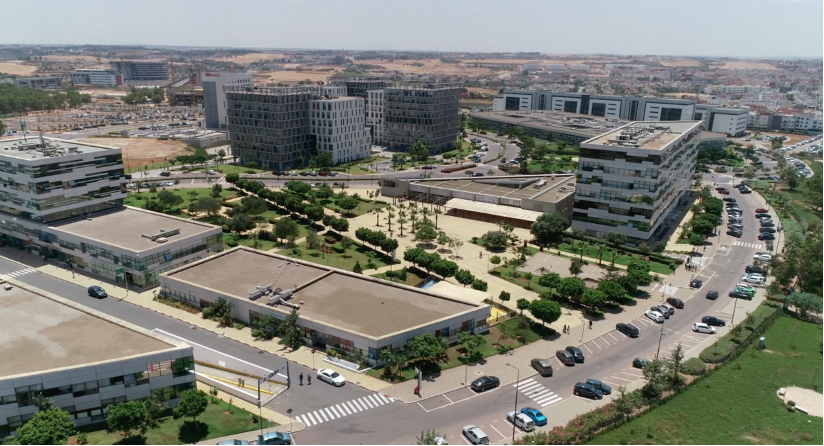
\includegraphics{figures/madc_location}
  % once you have the actual figure file.
  \begin{figure}[h]
    \centering
    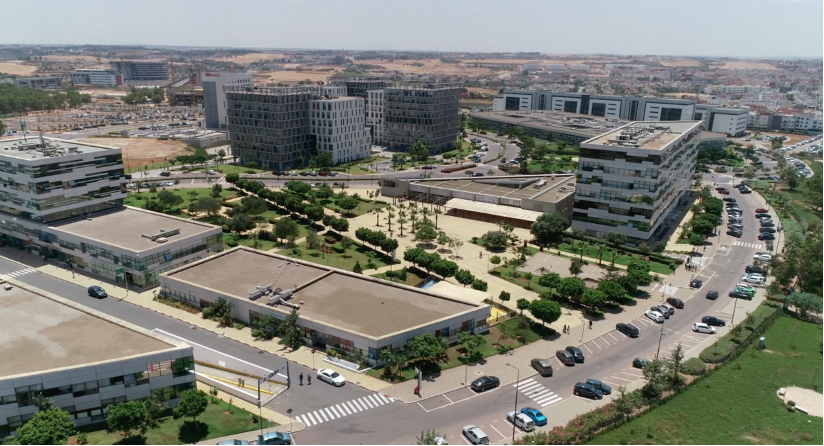
\includegraphics[width=0.8\textwidth]{figures/madc_location}
    \caption{Oracle MADC Location}
    \label{fig:madc_location}
  \end{figure}

  The first Oracle R\&D center in Africa and one of only a few globally, the
  Oracle Research \& Development Center Morocco is a software development center
  established by Oracle Corporation in Casablanca, Morocco. The center was
  inaugurated in 2022 and is one of Oracle's key development centers in the
  EMEA region. The center is staffed by highly skilled and talented software
  developers, engineers, and project managers who work on a variety of projects
  across various Oracle product lines utilizing the newest trends in innovation,
  such as artificial intelligence, augmented/virtual/mixed reality, big data
  analytics, Blockchain, cloud computing, cybersecurity, internet of things,
  machine learning, mobile computing, and serverless computing.

  The center's researchers make use of all these technologies to tackle the most
  pressing problems facing business, science, and the public sector. Expansion
  of internship and graduate recruitment initiatives and joint research projects
  with regional universities are all part of this global program.

  Oracle MADC has been successful in delivering several high-quality products
  and solutions, such as Oracle Cloud Infrastructure (OCI), Autonomous Data
  Warehouse (ADW), etc.

  \begin{figure}[h]
    \centering
    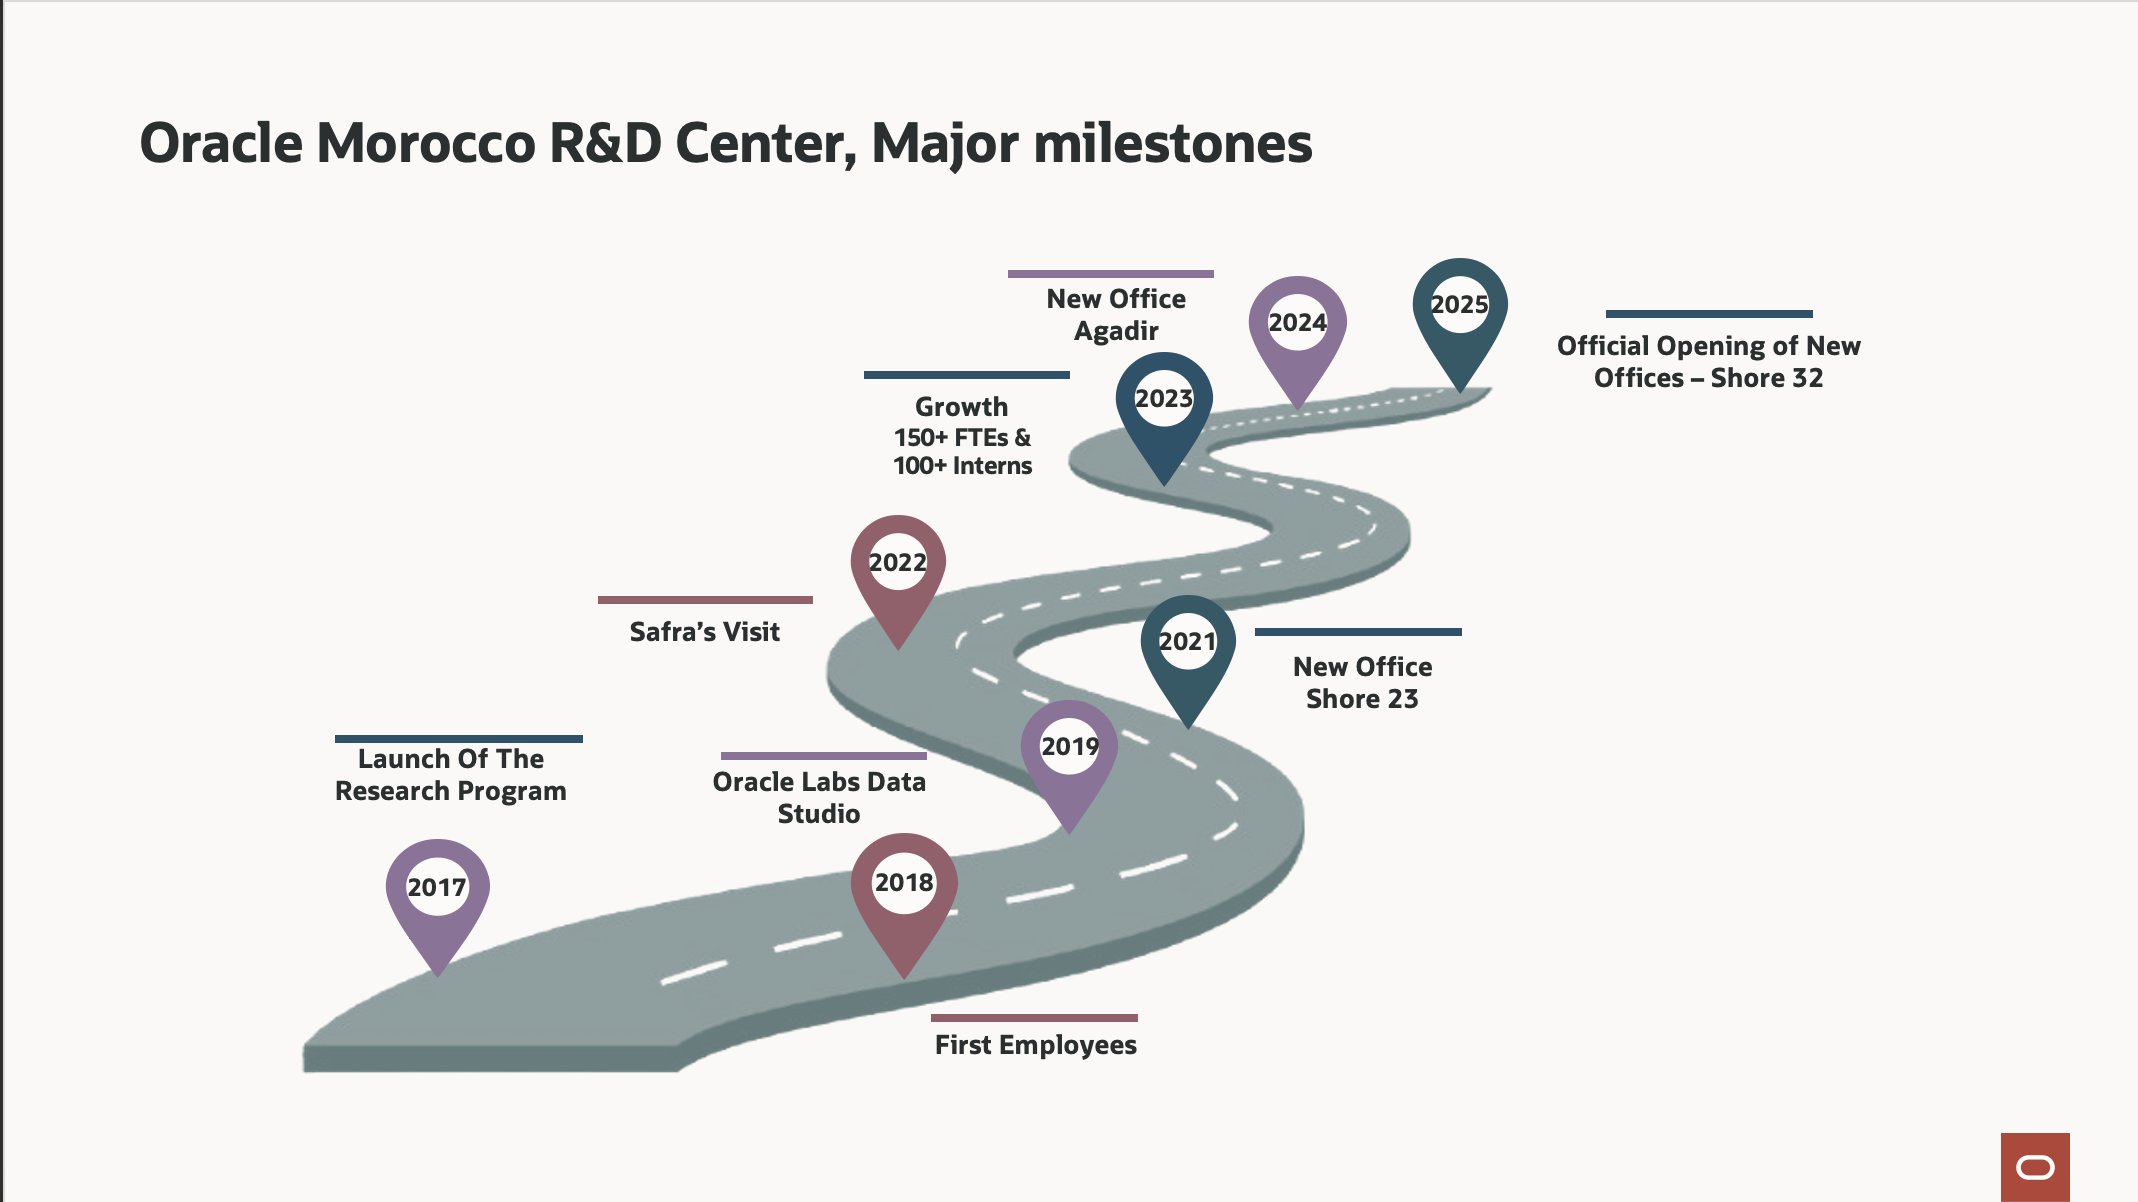
\includegraphics[width=0.8\textwidth]{figures/madc_milestones}
    \caption{MADC Major Milestones}
    \label{fig:madc_milestones}
  \end{figure}

  % ── 1.2.3 ──
  \subsection{Business Area of Activity}

  Oracle provides a variety of goods and services to its clients. Software
  development tools, cloud services, training, consultancy, and credentials are
  just a few of the goods and services offered. One of the brands Oracle offers
  is Oracle Database, which has held the top spot since 1979 and is supported
  by cloud artificial intelligence. SaaS, PaaS, IaaS, and DaaS are just a few
  of the integrated solutions offered by Oracle Cloud Infrastructure for
  business, IT, and development needs. Oracle Middleware is a platform
  integrated for creating and running intelligent, agile applications while
  increasing technical efficiency using contemporary software designs. Oracle
  Services include Oracle Advanced Customer Support Services, Oracle Premium
  Support, Oracle Consulting, Oracle Financing, and Oracle Managed Cloud Services.

    % ── 1.2.3.1 ──
    \subsubsection{Oracle Morocco R\&D Center Lines of Businesses (LOBs)}

      \paragraph{Oracle APEX}
      The most widely used enterprise low-code application platform in the world,
      Oracle APEX lets you create safe, scalable, and feature-rich web and mobile
      apps that can be deployed on-premises or in the cloud. With APEX, developers
      can create and launch engaging applications that address practical issues and
      deliver benefits right away. It is not necessary to possess extensive
      knowledge of multiple technologies to provide complex solutions.

      \paragraph{Oracle Health and Artificial Intelligence}
      Oracle APEX helps transform the technologies that are revolutionizing
      healthcare. Oracle APEX solutions accelerate the development of the next
      generation of drugs, devices, and therapies through a cohesive ecosystem
      that harnesses data to deliver results. There are no more silos --- just
      clinical trials, data, strategy, and insights flowing together for better
      outcomes.

      \paragraph{Oracle Linux}
      Oracle Linux delivers the operating system of choice for Oracle customers,
      Oracle Cloud, and Oracle Engineered Systems. Oracle has been an active
      contributor since 1998, shipping the first-ever commercial database on Linux
      along with multiple enhancements. Today, it is focused on developing
      open-source products while improving the stability and performance of the
      operating system.

      \paragraph{Oracle NetSuite}
      NetSuite is a cloud-based business management software that helps
      organizations manage their financials, operations, and customer
      relationships. It offers features such as accounting, CRM, inventory
      management, e-commerce, and more, all in one platform.

      \paragraph{Oracle Database Development Tools}
      The cloud and on-premises solutions drive the secure data access at a scale
      that powers the modern world. Combined with advanced data visualization and
      analysis, Oracle Database Development Tools enable data platforms for
      application development for any purpose. The products include Oracle SQL
      Developer, Oracle Data Modeler, Oracle REST Data Services, and Oracle SQLcl.

      \paragraph{Fusion ERP}
      Oracle Fusion Cloud ERP is a complete, modern, cloud ERP suite that provides
      teams with advanced capabilities, such as AI to automate manual processes,
      analytics to react to market shifts in real-time, and automatic updates to
      stay current and gain a competitive advantage.

      \paragraph{Oracle Analytics}
      Oracle Analytics is a comprehensive platform for diverse data workloads. It
      turns information into action with insights from cloud, on-premises, and
      hybrid data, empowering users to make business-defining decisions sooner
      through AI and ML-powered analytical applications.

      \paragraph{Oracle Cloud Infrastructure}
      Oracle Cloud is the first public cloud built from the ground up to be a
      better cloud for every application. By rethinking core engineering and
      systems design for cloud computing, it created innovations that solve
      problems customers have with existing public clouds and offers the complete
      services customers need to build innovative cloud applications.

      \paragraph{Oracle Digital Government Group}
      The data intelligence platform provides the insights that government leaders
      need to make the decisions that matter. The mission is to help national
      governments on their digital transformation journeys and improve citizens'
      experience with government services.

      \paragraph{Oracle Java Platform Group}
      The Oracle Java Platform Group is dedicated to advancing and maintaining the
      Java platform, a cornerstone of modern software development used by millions
      of developers worldwide. This group drives innovations in the Java ecosystem,
      ensuring the language remains robust, efficient, and versatile for a wide
      range of applications.

  % ── 1.2.4 ──
  \subsection{Organizational Structure}

  Oracle Corporation has a hierarchical organizational structure with three main
  business divisions: Hardware, Services, Cloud, and License. Each segment is
  divided into smaller business units focused on goods, services, or geographical
  areas. The Board of Directors oversees the company's performance and strategic
  direction, while the Executive Leadership Team manages daily operations.
  Functional divisions, including sales, marketing, finance, human resources,
  legal, and IT, fall under the Executive Leadership Team.

  Business units are arranged by region, product, and service, with a senior VP
  or general manager overseeing each unit's operations. The employees are
  subordinated to both a functional manager and a business unit manager in the
  matrix-based organizational structure of the business units.

  In general, Oracle's organizational structure is built to encourage teamwork,
  creativity, and client attention. The matrix form enables people to work across
  many functions and business divisions to achieve shared goals, while the
  hierarchical structure promotes effective decision-making and communication.

  % ── 1.2.5 ──
  \subsection{Organizational Culture}

  Oracle has a strong corporate culture that prioritizes innovation, client focus,
  and excellence. The company's history of innovation, emphasis on customer
  satisfaction, and dedication to fostering a friendly and collaborative work
  environment all shape the company's culture.

  Oracle's culture places a strong emphasis on the following values:

  \begin{description}
    \item[\textbf{Innovation}] One of Oracle's defining characteristics. The
    business has a lengthy history of creating cutting-edge goods and technology
    that have revolutionized the tech sector, promoted by a dedication to R\&D
    and by giving staff members the tools to test fresh concepts.

    \item[\textbf{Customer Satisfaction}] Oracle's customer-centric approach
    reflects its commitment to providing goods and services that satisfy client
    needs. Employees are encouraged to collaborate closely with clients to
    comprehend their demands and create tailored solutions.

    \item[\textbf{Quality}] Oracle is dedicated to providing quality operations,
    products, and services, reflected in its solid reputation for dependability
    and performance. The company expects every person to strive for excellence.

    \item[\textbf{Collaboration and Teamwork}] Effective collaboration is
    essential for achieving Oracle's goals. The company encourages employees to
    work together across departments and functions, providing tools and resources
    to facilitate communication.
  \end{description}

  Overall, Oracle's organizational culture is characterized by a commitment to
  innovation, customer focus, excellence, collaboration, and teamwork. These
  values are reflected in the company's products, services, and operations, and
  are embraced by its employees at all levels of the organization.

% ──────────────────────────────────────────
\section{Topic Context}
% ──────────────────────────────────────────

\subsection{General Context of the Project}

Before diving into the core issue of the topic, it is useful to provide some
background information. The team I worked with during this internship was called
``Digital Government'' --- which directly reflects the primary objective this
project aims to serve.

Digital government services --- also referred to as e-government --- refer to
the use of information and communication technologies to improve the efficiency,
effectiveness, and transparency of government operations. These systems reduce
bureaucratic delays, minimise paperwork, and enhance the overall quality of
public services.

E-government systems are commonly categorised based on the type of interaction
they facilitate. Three main categories exist: Government-to-Government (G2G),
Government-to-Citizen (G2C), and Government-to-Employee (G2E).

G2G refers to interactions between different government agencies or departments,
whether at the same level or across levels of government. An example relevant to
this project is the sharing of agricultural satellite data between a national
space agency and a ministry of agriculture to inform food security decisions.

G2C focuses on delivering government services and information directly to
citizens --- making them more accessible, timely, and actionable. In the context
of agriculture, this translates to providing smallholder farmers and local
administrations with accurate, up-to-date crop production intelligence.

G2E refers to internal government process management and employee communication
--- for example, equipping field agents with data-driven tools to support their
monitoring activities.

The Digital Government team at Oracle aims to leverage existing government data
and modern technologies to solve real-world problems across sectors including
agriculture, healthcare, and education. This project sits firmly within the
agricultural domain and contributes to Oracle's Government Data Intelligence for
Agriculture platform --- launched in September 2025 --- which supports
governments in building more resilient and data-driven food systems.

It is important to note that this project is part of an ongoing collaboration
with different governments. The requirements and needs of each country differ,
and Rwanda represents one of the early adopters of this approach.

\subsection{Problematic}

During my internship, my focus was on developing a machine learning pipeline to
classify crop types across Rwanda using Sentinel-2 satellite time series data
--- with the broader aim of supporting agricultural monitoring and food security
decision-making.

Agriculture plays a vital role in Rwanda's economy and food system. Accurate,
timely knowledge of what crops are growing where --- and how much --- is
essential for effective resource allocation, early warning of food shortfalls,
and informed policy decisions. However, obtaining this information at national
scale through traditional ground surveys is physically and financially
impossible. Surveys are expensive, sparse, seasonal, and always outdated by the
time results are available.

The challenge is compounded by the nature of smallholder agriculture in Rwanda.
Farms are small, fragmented, and often intercropped --- with multiple crops
growing on the same plot within the same season. Satellite pixels at the
boundary between fields capture mixed spectral signals from more than one crop,
creating label ambiguity. Cloud cover --- persistent throughout Rwanda's growing
seasons --- introduces temporal gaps in satellite observations that must be
handled carefully. And the extreme class imbalance between dominant crops and
minority crops like Sweet Potato --- representing only 0.3\% of the training
data --- makes reliable multi-class classification a significant methodological
challenge.

\subsection{Solution}

To address these challenges, I designed and implemented an end-to-end
multi-class crop classification pipeline using Sentinel-2 satellite time series
data, processed on Oracle Cloud Infrastructure.

The pipeline begins with rigorous data preprocessing --- including label noise
correction, boundary pixel identification and removal, geometric quality
filtering, cloud-based quality flagging, temporal gap analysis, and linear
interpolation to reconstruct missing observations. Each step was grounded in
peer-reviewed literature and validated against the data.

Eight vegetation indices were computed from the cleaned time series ---
capturing greenness, soil-adjusted vegetation, chlorophyll content, and moisture
levels. From these, 50 summary features were extracted per pixel: 32
statistical features capturing the overall seasonal signal, and 18 phenological
features capturing crop growth timing --- start of season, end of season, peak,
amplitude, rate of increase, and integral.

Feature selection was applied in three stages --- ANOVA, Random Forest
importance ranking, and Recursive Feature Elimination --- reducing the feature
set from 50 to 37 without loss of predictive performance. Class imbalance was
addressed through a combination of balanced class weights, SMOTE oversampling of
the minority class, and prediction threshold adjustment --- all optimised
through grid search.

Two models were trained and compared: Random Forest as a baseline and XGBoost
as the primary model. XGBoost outperformed Random Forest across all evaluation
metrics --- Macro F1, Weighted F1, G-mean, and Cohen's Kappa --- with
particularly significant gains on Sweet Potato classification, where F1
improved from 0.35 to 0.64.

This approach demonstrated that reliable multi-class crop mapping is achievable
from free satellite data at national scale --- with no field surveys required
--- and provides a foundation for integration into Oracle's Government Data
Intelligence for Agriculture platform.

% ──────────────────────────────────────────
\section{Conclusion}
% ──────────────────────────────────────────

This chapter introduced the general context of the internship project. It first
presented Oracle as the host organization, including its activities, structure,
culture, and the role of the Oracle Morocco Research and Development Center.
It then described the Digital Government context in which the project was
conducted, highlighting the importance of e-government services and their role
in improving public-sector decision-making.

The chapter also presented the main problem addressed during the internship:
the difficulty of producing accurate and timely crop-type information at
national scale using traditional field-survey methods. Finally, it introduced
the proposed satellite-based machine learning solution, which aims to support
agricultural monitoring and food security decision-making in Rwanda.